\chapter{轴向拉伸与压缩}
\intro{
	如果作用在物体一小块区域上的力系被另一个静力等效的力系所代替，那么这种代替只会在近处产生显著影响，而在离加力作用区稍远的地方，物体的应力分布几乎不受影响。
	
	\rightline{——Saint-Venant}
}
\begin{definition}
	作用在杆件两端的外力合力的作用线与杆件轴线重合。杆件的变形沿轴线的方向伸长或者缩短。
\end{definition}
\begin{figure}[htbp]
	\centering
	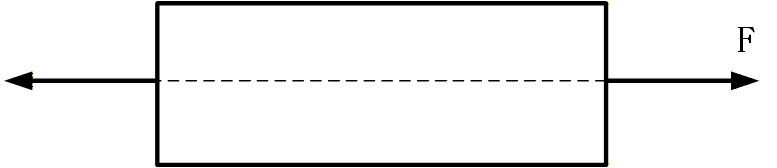
\includegraphics[width=0.5\linewidth]{Figure/轴向拉压力.png}
\end{figure}
\begin{definition}
	轴力：轴横截面上的内力。
	
	拉正压负。
\end{definition}

\section{斜截面上的应力}
\begin{definition}
	正应力：	$\sigma_{\alpha}=\sigma \cos^2 \alpha$
	
	切应力：	$\tau_{\alpha}=\frac{\sigma}{2}\sin 2\alpha$
\end{definition}
\begin{figure}[htbp]
	\centering
	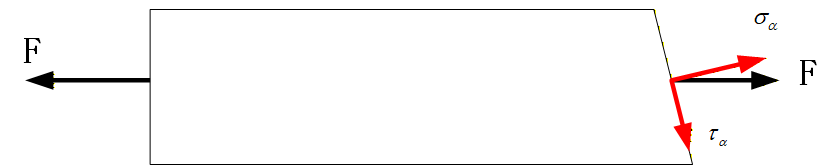
\includegraphics[width=0.6\linewidth]{Figure/应力分解.png}
\end{figure}
\begin{proof}
	\begin{align*}
		F_N=P_{\alpha}A_{\alpha}\\
		A=A_{\alpha}\cos{\alpha}\\
		\sigma_{\alpha}=P_{\alpha}\cos{\alpha}=\frac{F_N}{A}\cos^2 \alpha=\sigma\cos^2 \alpha\\	
		\sigma_{\alpha}=P_{\alpha}\sin{\alpha}=\frac{F_N}{A}\cos\alpha \sin\alpha=\frac{\sigma}{2}\sin 2\alpha
	\end{align*}
\end{proof}
	
\section{材料拉伸时的力学性能}
通过实验，我们可以得到材料的$F-\Delta l$曲线

\subsection{塑性材料拉伸时的力学性能}
\begin{figure}[htbp]
	\centering
	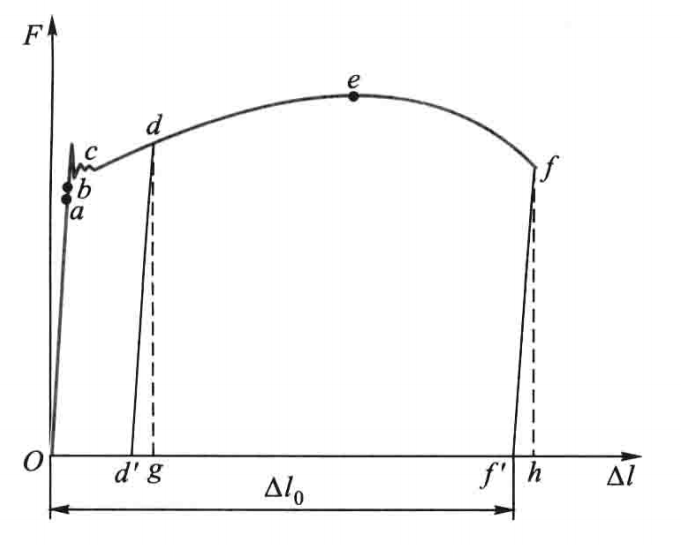
\includegraphics[width=0.6\linewidth]{Figure/低碳钢的拉伸曲线.png}
	\caption{低碳钢拉伸时的$F-\Delta l$曲线}
\end{figure}
为了消除试样尺寸的影响，我们可以将$F-\Delta l$曲线转换为$\sigma-\varepsilon$曲线。
\begin{definition}
	应力：$\sigma=\frac{F}{A}$
	
	应变：$\varepsilon=\frac{\Delta l}{l_0}$
\end{definition}
\begin{figure}[htbp]
	\centering
	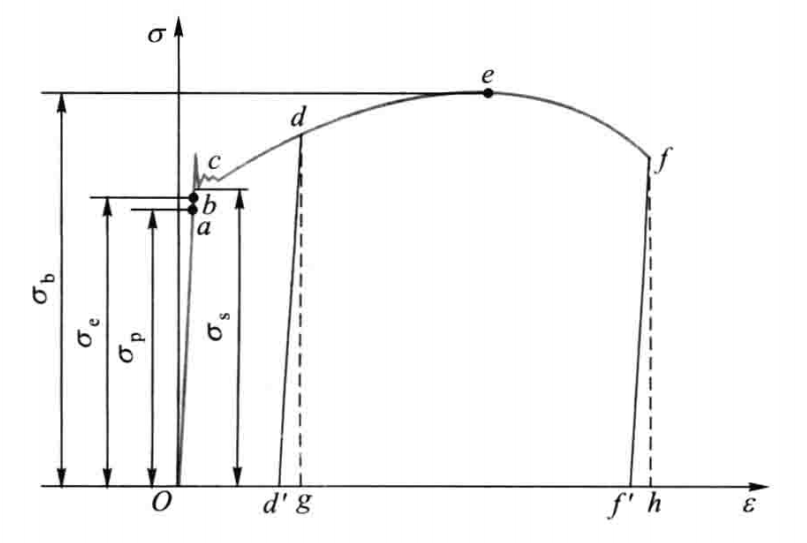
\includegraphics[width=0.6\linewidth]{Figure/5dac5636-fb99-4781-a8c8-ee10be6bdf8d.png}
	\caption{低碳钢拉伸时的$\sigma-\varepsilon$曲线}
\end{figure}

下面我们来分析一下$\sigma-\varepsilon$曲线的不同阶段。
\begin{itemize}
	\item 弹性阶段($0\to b$)：$\sigma$与$\varepsilon$成正比，满足Hooke定律$ \sigma = E \varepsilon $。
	\item 屈服阶段($b\to c$)：$\sigma$基本保持不变，$\varepsilon$继续增大。
	\begin{definition}
		屈服：材料在应力不增加的情况下发生较大塑性变形的现象。

		屈服强度或屈服极限$\sigma_s$:屈服阶段内最小的应力值。
	\end{definition}
	\item 强化阶段($c\to d$)：$\sigma$继续增大，$\varepsilon$继续增大。
	\begin{definition}
	强化：材料在屈服阶段后，随着应变的增大，所能承受的应力继续增大的现象。

	极限强度$\sigma_b$:强化阶段内最大的应力值。 
	\end{definition}
	\item 颈缩阶段($d\to e$)：$\sigma$达到最大值后开始下降，$\varepsilon$继续增大。
	\item 断裂阶段($e\to f$)：$\sigma$继续下降，$\varepsilon$继续增大，直到试样断裂。
	\begin{definition}
		断裂：材料在应力作用下发生破坏的现象。

		断后伸长率$\delta$:断裂阶段内试样的伸长率。$\delta=\frac{l_f-l_0}{l_0}\times 100\%$

		断面收缩率$\psi$:断裂阶段内试样的断面收缩率。$\psi=\frac{A_0-A_f}{A_0}\times 100\%$
	\end{definition}
\end{itemize}
\begin{definition}
	弹性模量$E$:弹性阶段内的应力与应变的比值。$E=\frac{\sigma}{\varepsilon}$
\end{definition}
\begin{definition}
	卸载定律：在弹性阶段内，材料的卸载曲线与加载曲线重合。

	冷作硬化：在塑性阶段内，材料的卸载曲线与加载曲线不重合，卸载曲线的斜率大于加载曲线的斜率。冷作硬化后，材料的屈服强度和极限强度都增加了。但是，冷作硬化会降低材料的塑性。
\end{definition}

\subsection{脆性材料拉伸时的力学性能}
\begin{figure}[htbp]
	\centering
	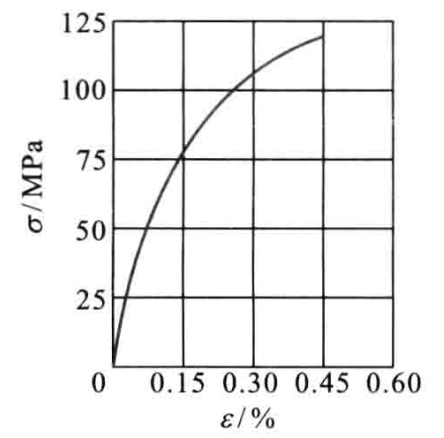
\includegraphics[width=0.6\linewidth]{Figure/铸铁的拉伸曲线.png}
	\caption{铸铁拉伸时的$F-\Delta l$曲线}
\end{figure}
可以看到，铸铁拉伸时的曲线没有明显的直线部分。弹性模量$E$随着应力的变化而变化。

显然，铸铁不抗拉。

\section{材料压缩时的力学性能}
脆性材料抗压不抗拉。

\section{拉压杆的强度条件}
\subsection{许用应力}
\begin{definition}
	塑性材料的许用应力：$[\sigma]=\frac{\sigma_s}{n}$

	n：安全系数。
\end{definition}

\begin{definition}
	脆性材料的许用应力：$[\sigma]=\frac{\sigma_b}{n}$

	n：安全系数。
\end{definition}

\subsection{强度条件}
$$\sigma_{max}=\frac{F_N}{A}\leq[\sigma]$$

\section{拉压杆的变形}
\subsection{轴向变形}
$\Delta l=l_1-l_0$

由Hooke定律，

$\Delta l=\frac{F_Nl_0}{EA}$

\subsection{横向变形}
\begin{definition}
	泊松比$\mu$:材料在拉伸时，横向变形与轴向变形的比值。$\mu=\frac{\Delta l_{\alpha}}{\Delta l}$

\end{definition}


\section{拉、压超静定问题}
一般步骤：
\begin{enumerate}
	\item 列出独立的平衡方程
	\item 找出变形几何关系（以切代弧）
	\item 找出物理关系（Hooke定律）
	\item 解决问题
\end{enumerate}

\section{拉压时的应变能}
\begin{definition}
	应变能：固体在外力作用下，因变形而存储的能量。
\end{definition}
应变能：
\begin{align*}
	V_s=\frac{1}{2}F\Delta l\\
	=\frac{F_N^2l}{2EA}
\end{align*}

应变能密度：
\begin{align*}
	 v_s=\frac{V_s}{V}\\
	 =\frac{1}{2}E\varepsilon^2\\
	 =\frac{1}{2}\sigma \varepsilon
\end{align*}
\section{应力集中}
在构件尺寸突变处，会发生应力局部增大的现象，称为\textbf{应力集中}。在进行工程设计时，需要考虑该效应对强度的影响。


